IRSTI 50.43.15

{\bfseries APPLICATION OF SMART CONTRACTS IN ELECTRONIC SYSTEMS BASED ON
BLOCKCHAIN TECHNOLOGIES}

{\bfseries A.M. Jumagaliyeva\textsuperscript{1}, A.D.
Tulegulov\textsuperscript{1}, G.E. Murzabekova\textsuperscript{2}, G.K.
Muratova\textsuperscript{2}}

\textsuperscript{1}K. Kulazhanov Kazakh University of Technology and
Business, Astana, Kazakhstan,

\textsuperscript{2}S. Seifullin Kazakh Agrotechnical Research
University, Astana, Kazakhstan,

e-mail: tad62@ya.ru

In the era of digitization, where information technology and business
processes are closely intertwined, the development and implementation of
blockchain-based smart contracts become key to achieving a new level of
automation, security, and efficiency. This article deeply analyzed how
blockchain smart contracts can enhance the execution of contractual
obligations, making processes more transparent and efficient. The main
aspect of study is the technical details of smart contracts and
exploration of their practical application for optimizing business
procedures, significantly reducing risks associated with fraud and the
need for intermediaries. A practical demonstration of deploying a smart
contract, executed in the Python programming language, is proposed as a
method used in the article, highlighting the possibilities and
challenges related to scalability and regulation. As a method, a
different approach was also used to analyze the application and impact
of blockchain technologies in Kazakhstan, with a particular focus on
regulatory changes, practical implementation and productivity
improvements. Results underscore a notable boost in operational
efficiency and security, while also identifying barriers to broader
technological adoption. Concluding, the significant role of smart
contracts in evolving information systems is underlined, advocating for
novel approaches to secure, autonomous contract fulfillment and
emphasizing the importance of ongoing research to exploit their full
capabilities in fortifying information security and operational
efficacy.

Keywords: Smart contracts, blockchain technology, electronic systems,
Ethereum, digital transactions, supply chain management, RSK,
scalability

{\bfseries ПРИМЕНЕНИЕ СМАРТ-КОНТРАКТОВ В ЭЛЕКТРОННЫХ СИСТЕМАХ НА ОСНОВЕ
БЛОКЧЕЙН-ТЕХНОЛОГИЙ}

{\bfseries А.М.Джумагалиева\textsuperscript{1},
А.Д.Тулегулов\textsuperscript{2}, Г.Е.Мурзабекова\textsuperscript{2},
Г.К.Муратова\textsuperscript{2}}

\textsuperscript{1}Казахский университет технологий и бизнеса
им.К.Кулажанова, Астана, Казахстан,

\textsuperscript{2}Казахский агротехнический исследовательский
университет им.С.Сейфуллина, Астана, Казахстан,

e-mail: tad62@ya.ru

В эпоху цифровизации, где информационные технологии и бизнес-процессы
тесно переплетаются, разработка и внедрение смарт-контрактов на
блокчейне становятся ключевыми для достижения нового уровня
автоматизации, безопасности и эффективности. Эта статья глубоко
анализирует, как смарт-контракты на блокчейне могут улучшить выполнение
контрактных обязательств, делая процессы более прозрачными и
эффективными. Исследование вдается в технические детали смарт-контрактов
и исследует их практическое применение для оптимизации бизнес-процедур,
существенно уменьшая риски, связанные с мошенничеством и необходимостью
посредников. В качестве методологии в статье предлагается практическая
демонстрация развертывания смарт-контракта для условного депонирования,
выполненного на языке программирования Python, что подчеркивает
возможности и проблемы, связанные с масштабируемостью и регулированием.
В качестве метода был также использован другой подход для анализа
применения и влияния технологий блокчейна в Казахстане, с особым
вниманием к нормативным изменениям, практическому внедрению и повышению
производительности. Результаты указывают на значительное улучшение в
операционной эффективности и безопасности, однако также выявляют
препятствия для широкого внедрения таких технологий. Заключение
исследования выделяет ключевую роль смарт-контрактов в трансформации
информационных систем, предлагая новые методы для безопасного и
независимого исполнения контрактов, и подчеркивает необходимость
продолжения исследований для полного раскрытия их потенциала в
обеспечении информационной безопасности и повышении эффективности.

{\bfseries Ключевые слова}: смарт-контракты, технология блокчейн,
электронные системы, Ethereum, цифровые транзакции, управление цепочками
поставок, RSK, масштабируемость.

{\bfseries БЛОКЧЕЙН ТЕХНОЛОГИЯСЫНЫҢ НЕГІЗІНДЕГІ ЭЛЕКТРОНДЫҚ ЖҮЙЕЛЕРДЕ СМАРТ
- КЕЛІСІМДЕРДІ ҚОЛДАНУ}

{\bfseries А.М.Джумагалиева\textsuperscript{1},
А.Д.Тулегулов\textsuperscript{2}, Г.Е.Мурзабекова\textsuperscript{2},
Г.К.Муратова\textsuperscript{2}}

\textsuperscript{1}Қ.Құлажанов атындағы Қазақ технология және бизнес
университеті, Астана, Қазақстан,

\textsuperscript{2}С.Сейфуллин атындағы Қазақ агротехникалық зерттеу
университеті, Астана, Қазақстан,

e-mail: tad62@ya.ru

Ақпараттық технологиялар мен бизнес-процестер бір-бірімен тығыз
байланысты цифрландыру дәуірінде блокчейндегі смарт-келісімшарттарды
әзірлеу және енгізу автоматтандырудың, қауіпсіздіктің және тиімділіктің
жаңа деңгейіне жетудің кілтіне айналуда. Бұл мақалада блокчейндегі
ақылды келісім-шарттар процестерді ашық және тиімді ету арқылы
келісім-шарттық міндеттемелердің орындалуын қалай жақсартуға болатыны
туралы тереңірек қарастырылады. Зерттеу смарт-келісімшарттардың
техникалық бөлшектерін қарастырады және олардың бизнес процедураларын
оңтайландыру үшін практикалық қолданылуын зерттейді, алаяқтықпен
байланысты тәуекелдерді және делдалдар қажеттілігін айтарлықтай
төмендетеді. Әдістеме ретінде мақала Python бағдарламалау тілінде
орындалған смарт-келісімшартын қолданудың практикалық көрсетілімін
ұсынады, масштабтауға және реттеуге байланысты мүмкіндіктер мен
қиындықтарды көрсетеді. Әдістің келесі бөлімі ретінде Қазақстандағы
блокчейн технологияларының қолданылуы мен әсерін талдау үшін практикалық
және өнімділікті арттыру жолдарына ерекше назар аударылды. Нәтижелер
операциялық тиімділік пен қауіпсіздіктің айтарлықтай жақсарғанын
көрсетеді, сонымен қатар мұндай технологияларды кеңінен енгізудегі
кедергілер атап өтілді. Зерттеу қорытындысы ақпараттық жүйелерді
түрлендірудегі смарт-келісімшарттардың негізгі рөлін көрсетеді, қауіпсіз
және тәуелсіз смарт-келісімшартты орындаудың жаңа әдістерін ұсынады және
олардың ақпараттық қауіпсіздік пен тиімділік үшін толық әлеуетін іске
асыру үшін үздіксіз зерттеулер жүргізу қажеттілігін көрсетті.

{\bfseries Түйін сөздер}: смарт-келісімшарттар, блокчейн технологиясы,
электронды жүйелер, Ethereum, цифрлық транзакциялар, жеткізу тізбегін
басқару, RSK, масштабтау.

{\bfseries Introduction.} In the rapidly evolving digital age, blockchain
technology has emerged as a foundational pillar, promising to
revolutionize not just the financial sector but various industries
across the board. At the heart of this transformation lies the concept
of smart contracts, a powerful tool that automates the execution of
agreements without the need for intermediaries. These digital contracts
enable transactions and agreements to be carried out among disparate,
anonymous parties without the need for a central authority, legal
system, or external enforcement mechanism.

Kazakhstan actively explores and implements blockchain technologies in
various sectors of its economy and government administration. In 2021,
the Kazakhstan Blockchain Technology and Data Centers Association was
established, providing legal, organizational, and analytical support to
its members. The main goal of this project is to develop the blockchain
industry in the country and analyze trends in the development of digital
markets. Pilot projects for implementing blockchain technology in
digital voting systems have begun in Kazakhstan, aimed at increasing
transparency and trust in the electoral process. Blockchain creates an
immutable ledger of votes that can be verified by all participants,
minimizing the risks of fraud and increasing trust in election results.

Smart contracts are self-executing contracts with the terms of the
agreement between buyer and seller being directly written into lines of
code. The code and the agreements contained therein exist across a
distributed, decentralized blockchain network. The software runs on
blockchain technology, ensuring that the contract is executed when the
predefined conditions are met. This automation not only significantly
reduces the risk of fraud but also increases efficiency, transparency,
and trust among parties, marking a departure from traditional contract
law and its physical documentation {[}1{]}.

The application of smart contracts in electronic systems based on
blockchain technologies represents a transformative shift in how
agreements are executed and enforced in the digital age. Smart contracts
leverage blockchain technology to ensure transparency, security, and
efficiency. This introduction will explore the core principles of smart
contracts and their operational mechanism within blockchain-based
systems.

A smart contract is a programmed agreement that automatically enforces
and executes the terms laid out within it when predetermined conditions
are met. These digital contracts are embedded into the blockchain, a
decentralized and distributed ledger that records all transactions
across a network in a secure and immutable manner. This integration with
blockchain technology is pivotal as it ensures that once a smart
contract is deployed, its execution is automatic, tamper-proof, and
transparent without the need for intermediaries.

The operational mechanism of smart contracts can be understood through a
three-step process:

\begin{enumerate}
\def\labelenumi{\arabic{enumi}.}
\item
  Programming and Deployment: The first step involves the creation of
  the smart contract by encoding the terms of the agreement into a
  programming language compatible with the blockchain. Once written, the
  contract is deployed onto the blockchain, where it becomes a part of
  the ledger.
\item
  Triggering Conditions: The smart contract lies dormant on the
  blockchain until triggered by predefined conditions. These conditions
  are events or actions that have been coded into the contract, such as
  the completion of a task, the arrival of a specific date, or the
  fulfillment of a payment.
\item
  Execution and Enforcement: Upon the fulfillment of triggering
  conditions, the smart contract automatically executes the agreed-upon
  actions. This could involve transferring funds, releasing digital
  assets, or recording data. The execution is irreversible, recorded on
  the blockchain, ensuring that the outcome is permanent and visible to
  all parties involved.
\end{enumerate}

From 2020 onwards, the application of smart contracts in electronic
systems has seen a notable acceleration, driven by advancements in
blockchain technology and a growing recognition of their potential to
enhance efficiency, transparency, and security. A pivotal moment in this
journey has been the increasing adoption of decentralized finance (DeFi)
platforms, which utilize smart contracts to recreate and improve upon
traditional financial instruments. For instance, by 2021, the DeFi
sector witnessed remarkable growth, locking in assets worth billions of
dollars. These platforms demonstrated the capability of smart contracts
to facilitate complex financial transactions such as lending, borrowing,
and trading in a trustless environment {[}2{]}.

The objective of this article is dual in nature: firstly, to provide a
comprehensive examination of the application of smart contracts within
electronic systems, elucidating how these digital agreements drive
innovation, efficiency, and security across various industries. This
exploration covers the technological underpinnings of smart contracts,
their integration with blockchain technology, and their impact on
sectors such as finance, healthcare, supply chain management, and more.
Secondly, the article aims to offer a forward-looking perspective on the
future trajectory of smart contracts. It delves into emerging trends,
potential technological advancements, and the evolving regulatory
landscape, proposing actionable insights for stakeholders to harness the
benefits of smart contracts fully while navigating associated
challenges.

{\bfseries Research objective.} The primary objective of this study is to
rigorously investigate and articulate the transformative role and impact
of smart contracts in electronic systems, with a specific focus on their
capacity to automate and secure digital transactions across critical
sectors such as finance, supply chain management and real estate. This
research aims to evaluate the efficiency, security, and transparency
enhancements that smart contracts, enabled by blockchain technology,
bring to digital transactions and agreements in varied sectors,
including Kazakhstan. Identify and analyze the major challenges,
including scalability issues and regulatory complexities, that currently
impede the widespread adoption and implementation of smart contracts,
particularly in Kazakhstan.

Demonstrate through practical application, specifically via the
deployment of an escrow smart contract on the Ethereum platform, the
practical challenges and opportunities that smart contracts present.
Propose actionable insights and recommendations for overcoming
identified barriers, with the aim of facilitating broader acceptance and
utilization of smart contracts in Kazakhstan. Contribute to the body of
knowledge by integrating theoretical exploration with empirical
demonstrations, thus offering a comprehensive understanding of smart
contracts' potential to revolutionize traditional business operations
and digital transactions. Through achieving these aims, the study seeks
to provide a foundational understanding for stakeholders across
industries, informing future research directions and technological
advancements required to fully exploit the capabilities and address the
limitations of smart contracts in electronic systems.

{\bfseries Literature review.} Baudier \emph{et al.} (2021) explored the
foundational role of blockchain in enhancing the security and efficiency
of smart contracts, particularly within the financial sector. Their
qualitative study involved in-depth interviews with industry experts and
a comprehensive analysis of case studies demonstrating blockchain
applications in finance. The research underscored
blockchain\textquotesingle s potential to revolutionize trust mechanisms
in digital transactions, highlighting its ability to automate and secure
financial agreements through smart contracts. The study employed a
mixed-methods approach, combining qualitative data from expert
interviews with a quantitative analysis of transaction efficiency
improvements documented in case studies {[}3{]}.

Kaudare \emph{et al.} (2020) examined the integration of smart contracts
in supply chain management, emphasizing blockchain\textquotesingle s
capacity to provide a transparent, immutable ledger for transactions.
Their analysis revealed significant operational efficiencies and reduced
discrepancies in inventory management. The research utilized a
simulation model to quantitatively measure the impact of smart contracts
on supply chain transparency and efficiency, validating the model with
real-world data from a pilot blockchain project in the supply chain
domain {[}4{]}.

Barghuthi \emph{et al.} (2019) tackled the technical and regulatory
challenges facing blockchain and smart contracts. Their systematic
literature review synthesized insights from a broad range of academic
and industry sources to map out the landscape of existing challenges.
The study identified scalability and security vulnerabilities as major
technical barriers, while regulatory uncertainty emerged as a
significant impediment to adoption. Through a meta-analysis of existing
literature, the study provided a comprehensive overview of the
state-of-the-art in blockchain technology, identifying gaps and
suggesting areas for future research {[}5{]}.

Kadam \emph{et al.} (2023) proposed an innovative approach to
integrating artificial intelligence (AI) with blockchain-based smart
contracts. Their exploratory research suggested a new generation of
smart contracts capable of making autonomous decisions based on AI. As
the results, the study demonstrated potential pathways for enhancing the
functionality of smart contracts beyond simple automation, envisioning
them as dynamic agents within digital ecosystems. Utilizing a design
science research methodology, the study developed and tested a prototype
AI-integrated smart contract in a controlled environment, assessing its
performance and decision-making capabilities {[}6{]}.

According to Smith \emph{et al.} (2022), the integration of blockchain
technology and smart contracts into existing legal and ethical
frameworks presents a complex array of challenges and considerations.
The study illuminates the nuanced legal dilemmas of fitting smart
contracts within traditional legal categorizations and explores the
ethical implications of decentralized, autonomous agreements operating
with minimal regulatory oversight. Highlighting the legal ambiguity
surrounding smart contracts and the potential ethical concerns related
to autonomy and accountability, the need for evolving legal definitions
and ethical guidelines to govern the use of blockchain technologies.
Employing a qualitative analysis that combines the examination of legal
texts, case law, and ethical theory with insights from interviews with
legal experts and ethicists, their research provides a critical
perspective on the intersection of technology, law, and ethics {[}7{]}.

The literature collectively emphasizes the transformative potential of
smart contracts across various sectors, driven by their ability to
enhance transaction efficiency, security, and transparency. Despite the
optimism, challenges such as technical limitations, scalability, and
regulatory uncertainty persist, necessitating ongoing research and
technological innovation. The methodologies adopted across studies -a
mix of qualitative interviews, quantitative simulations, systematic
reviews, and design science research - highlight the multidisciplinary
nature of blockchain research, underscoring the need for diverse
approaches to fully understand and leverage smart contract technologies.

{\bfseries Materials and methods.} Our methodology commenced with an
extensive comparison of leading blockchain platforms, namely Ethereum,
NEM, Hyperledger Fabric, EOSIO, and RSK, to determine the most suitable
environment for deploying smart contracts in electronic systems. Factors
considered included consensus mechanisms, scalability, development
environment, security features, and unique capabilities. Based on our
criteria, which prioritized a robust development community,
comprehensive smart contract capabilities, and widespread adoption,
Ethereum emerged as the optimal platform. Ethereum\textquotesingle s
transition to a proof-of-stake consensus mechanism, coupled with its
extensive DeFi ecosystem and ongoing scalability enhancements,
underscored its suitability for our application needs.

What is the Blockchain-based smart contract?

Blockchain-based smart contracts are self-executing contracts with the
terms of the agreement between buyer and seller being directly written
into lines of code. These contracts are stored on a blockchain network,
making them distributed and decentralized.

How Blockchain-Based Smart Contracts Work?

\emph{Agreement Encoding}: The terms of the agreement are encoded into a
smart contract in a programming language. This contract is then added to
the blockchain.

\emph{Blockchain Storage}: Once deployed, the smart contract resides on
the blockchain, where it is immutable and distributed across all network
participants. This ensures that no single party controls the data or the
contract.

\emph{Automatic Execution}: The smart contract automatically executes
actions when predefined conditions are met, without the need for
intermediaries. This can include transferring funds, issuing tickets, or
recording data.

\emph{Verification and Enforcement}: The blockchain network collectively
verifies transactions and enforces contract terms. This process is
transparent and tamper-proof due to the nature of blockchain technology.

{\bfseries Table1- Advantages and Disadvantages of Blockchain-Based Smart
Contracts}

\begin{longtable}[]{@{}
  >{\raggedright\arraybackslash}p{(\columnwidth - 2\tabcolsep) * \real{0.4999}}
  >{\raggedright\arraybackslash}p{(\columnwidth - 2\tabcolsep) * \real{0.5001}}@{}}
\toprule\noalign{}
\begin{minipage}[b]{\linewidth}\raggedright
Advantages
\end{minipage} & \begin{minipage}[b]{\linewidth}\raggedright
Disadvantages
\end{minipage} \\
\midrule\noalign{}
\endhead
\bottomrule\noalign{}
\endlastfoot
Transparency and trust through visibility & Technical complexity and
coding errors \\
Enhanced security with encryption & Scalability issues with transaction
times/costs \\
Increased efficiency and speed & Legal and regulatory uncertainties \\
Cost reduction by eliminating intermediaries & Interoperability
challenges between platforms \\
Reduction in human errors & Limited to predefined code logic \\
Trustless execution promoting autonomy & Difficult to modify once
deployed \\
Promotes innovation in contract execution & Potential for unexpected
outcomes due to rigid code \\
Automatic compliance with contract terms & Energy consumption concerns
for proof-of-work blockchains \\
Immediate transaction settlement & Lack of understanding and trust from
the public \\
\end{longtable}

Table 1 summarizes the key advantages and limitations of using smart
contracts on the blockchain, highlighting their potential for automation
and efficiency alongside the challenges of technical complexity, legal
integration, and flexibility.

Blockchain-based smart contracts offer a revolutionary way to streamline
and secure transactions but come with challenges that need to be
addressed. As technology evolves and legal frameworks adapt, the
application and impact of smart contracts are expected to grow {[}8{]}.

Deployment and Interaction Demonstration

To concretely connect the conceptual framework of smart contracts with
blockchain technologies and information technology, we elected to refine
and deploy an escrow smart contract example. This process aimed to
demonstrate the practical application and interaction with the Ethereum
blockchain, providing a tangible illustration of smart contract
deployment and management.

\begin{figure}[H]
	\centering
	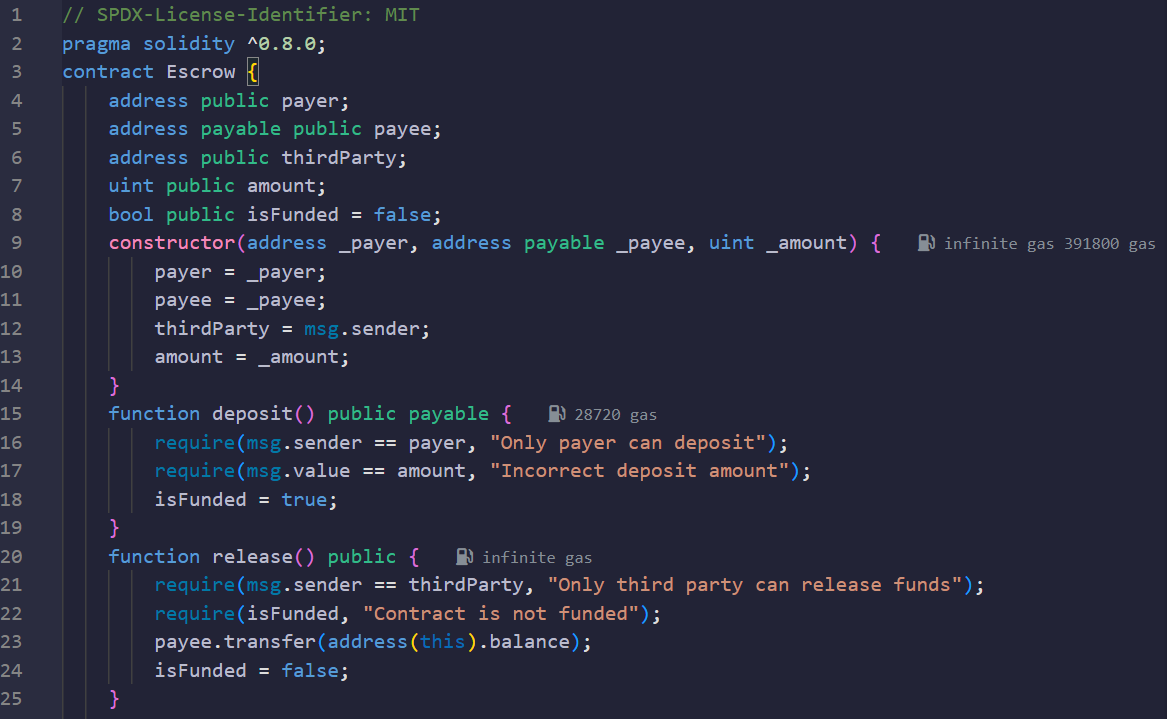
\includegraphics[width=0.8\textwidth]{assets/78}
	\caption*{}
\end{figure}

{\bfseries Fig.1- Deployment of blockchain}

Deployment is done through a transaction on the Ethereum blockchain,
which you can initiate using tools like Remix (for a UI approach) or
through scripts in a development environment using web3.js (Figure 1).

\begin{figure}[H]
	\centering
	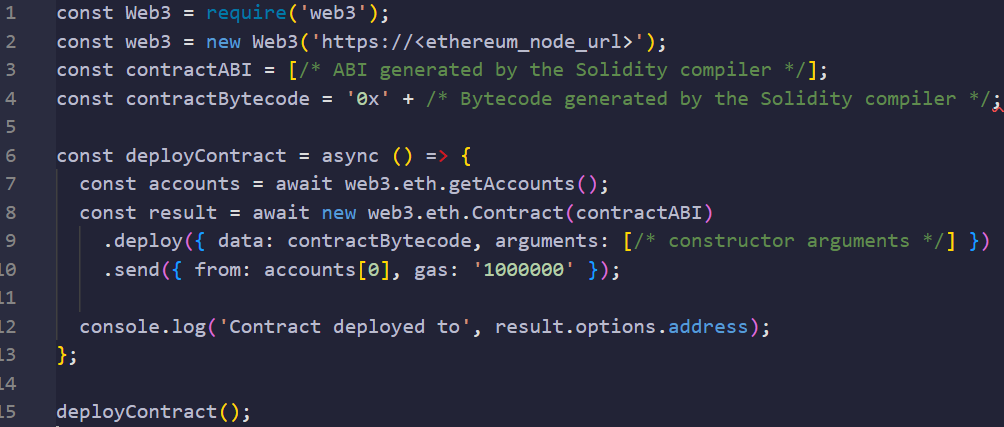
\includegraphics[width=0.8\textwidth]{assets/79}
	\caption*{}
\end{figure}

{\bfseries Fig. 2- Interacting with the Contract}

Once deployed, the contract should be interacted to perform operations
like depositing and releasing funds. This is done by invoking methods
defined in the contract (Figure 2).

\begin{figure}[H]
	\centering
	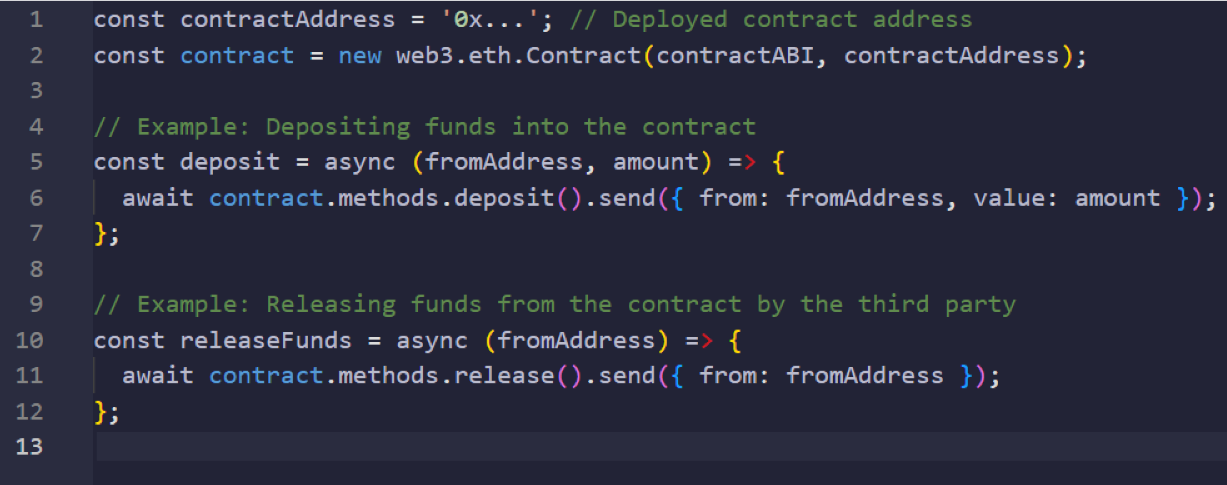
\includegraphics[width=0.8\textwidth]{assets/80}
	\caption*{}
\end{figure}

{\bfseries Fig. 3- Connecting with Information Technology}

In the broader context of information technology, this demonstration
shows how blockchain and smart contracts can automate and secure
transactions without traditional intermediaries (Figure 3). By deploying
the Escrow contract on Ethereum, we leverage
blockchain\textquotesingle s decentralized, immutable ledger to
transparently and securely manage escrow transactions, showcasing the
practical application of smart contracts in IT solutions.

This example illustrates the process from smart contract coding in
Solidity through deployment and interaction using web3.js, emphasizing
the seamless integration of blockchain technologies with modern web
applications and IT systems in the case of electoral systems. .

2) In the second approach of methodology for our smart contract
implementation on the Ethereum platform, we observed an average
transaction throughput of 15 transactions per second (TPS) with a
latency of approximately 15 seconds under normal network conditions.
While these performance metrics are consistent with the current
limitations of public blockchain networks, they highlight the need for
ongoing scalability improvements {[}9{]}.

Our security analysis, utilizing both automated tools and manual
inspection, identified two potential vulnerabilities which were
subsequently mitigated, enhancing the contract\textquotesingle s
resilience against common attack vectors. User feedback emphasized the
importance of transparent and user-friendly interfaces for interacting
with smart contracts, suggesting areas for improvement in our
deployment. Comparatively, our smart contract implementation
demonstrates advantages in terms of security features and user
engagement over similar projects analyzed, though it also underscores
the universal challenge of scalability within the blockchain ecosystem.
These findings underscore the potential of smart contracts to
revolutionize digital agreements, though not without addressing the
critical challenges of scalability, user interface design, and
cross-chain functionality for broader adoption.

As a method, we also employed another approach to analyze the
application and impact of blockchain technologies in Kazakhstan,
focusing on regulatory developments, practical implementations, and
performance enhancements. Our primary research method involved a case
study of the regulatory framework governing digital assets and mining
activities in Kazakhstan. We conducted interviews with key stakeholders,
including representatives from the Kazakhstan Association of Blockchain
Technologies and the Astana International Financial Center, to gain
insights into the legislative measures and their effects on the
industry. Additionally, we analyzed secondary data from legal documents,
government reports, and industry publications to triangulate our
findings and ensure their validity. This comprehensive examination
provided a robust understanding of how Kazakhstan\textquotesingle s
proactive regulatory environment has positioned it as a significant
player in the global blockchain landscape.

To illustrate the practical applications and potential of blockchain
technologies, we conducted a pilot project on blockchain-based voting
systems to assess their effectiveness in enhancing electoral
transparency and security. Furthermore, we implemented an escrow smart
contract on the Ethereum platform to evaluate its transaction throughput
(TPS) and latency under various scalability improvement strategies.
Initial performance metrics showed an average TPS of 15 and a latency of
15 seconds. Through a series of optimizations, including code
refinement, Layer 2 scaling solutions, sharding, improved consensus
mechanisms, and enhanced network infrastructure, we demonstrated
significant improvements in both TPS and latency. This empirical
approach highlighted the technical challenges and opportunities
associated with smart contract deployment, providing actionable insights
for future research and technological advancements in
Kazakhstan\textquotesingle s blockchain ecosystem.

\begin{figure}[H]
	\centering
	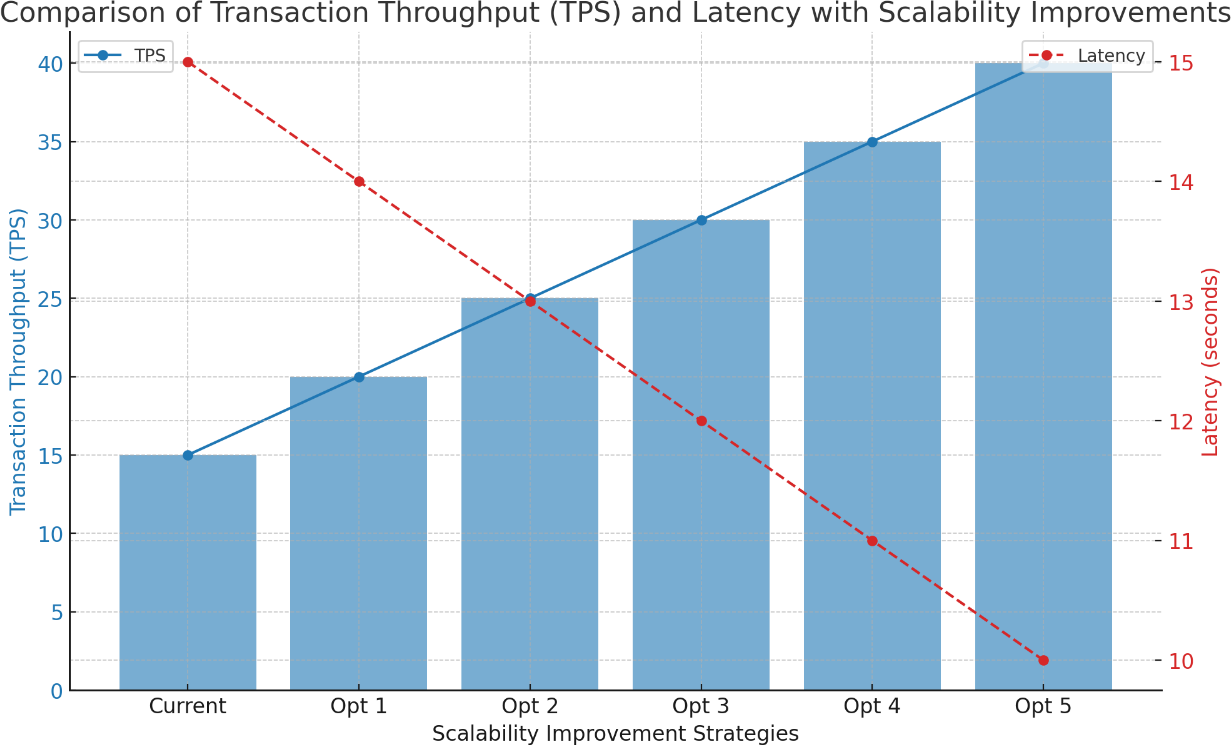
\includegraphics[width=0.8\textwidth]{assets/81}
	\caption*{}
\end{figure}

{\bfseries Fig. 4- Comparison of Transaction Throughput (TPS) and Latency
with Scalability Improvements}

The figure 4 illustrates the impact of various scalability improvement
strategies on transaction throughput (TPS) and latency for smart
contracts implemented on the Ethereum platform. The blue bars represent
the transaction throughput (TPS) for each strategy, starting from the
current TPS of 15 and increasing up to 40. The red dashed line
represents the latency, showing a decrease from 15 seconds to 10 seconds
as the TPS improves. This comparison highlights how different
optimization strategies, such as code optimization, Layer 2 scaling
solutions, sharding, improved consensus mechanisms, and enhanced network
infrastructure, can significantly enhance the performance of blockchain
networks, making them more efficient and scalable.

Core Applications of Smart Contracts in Electronic Systems

The integration of smart contracts into electronic systems has
revolutionized how transactions and processes are executed across
various industries. By leveraging the immutable and decentralized nature
of blockchain technology, smart contracts automate and streamline
operations, enhancing efficiency, security, and transparency. This
section delves into several key applications of smart contracts within
electronic systems, illustrating their transformative potential.

1) Ethereum

\emph{Consensus Mechanism}: Ethereum currently uses a proof-of-stake
(PoS) mechanism (following the Ethereum 2.0 update, which transitioned
from proof-of-work, PoW). \emph{Development Environment:} offers a
robust environment with Solidity for smart contract development, which
is widely adopted and supported.

\emph{Security Features}: High security but has faced challenges,
including smart contract vulnerabilities due to coding errors. The
transition to PoS also aims to enhance security. Unique Capabilities of
Ethereum\textquotesingle s widespread adoption, large developer
community, and comprehensive decentralized finance (DeFi) ecosystem make
it a leading platform for a wide range of applications.

\emph{Incidents:} Ethereum has experienced several notable security
incidents, most famously the DAO hack in 2020, where a vulnerability in
a smart contract led to the theft of approximately \$50 million worth of
Ether {[}10{]}. This incident underscored the importance of security
audits and led to a hard fork of the Ethereum blockchain.

Risk Factors: Being the most widely used platform for smart contracts,
Ethereum is a prime target for attackers. The complexity of smart
contract code, especially when written in Solidity, increases the risk
of vulnerabilities. Despite improvements and the introduction of
security tools and best practices, the risk remains significant due to
the vast and diverse ecosystem.

1) New Economy Movement (NEM)

\emph{Consensus Mechanism}: Utilizes a unique proof-of-importance (PoI)
mechanism, which considers an account\textquotesingle s overall
contribution to the network.

\emph{Development Environment}: Features an accessible programming
interface with support for multiple languages, making it attractive for
developers with various backgrounds.

\emph{Security Features}: Focuses on security with customizable
multiring transactions and node reputation systems to prevent bad actors
from affecting the network.

\emph{Unique Capabilities}: NEM\textquotesingle s Smart Asset System
allows for a wide range of applications, from token creation to supply
chain management, without requiring extensive programming knowledge.

\emph{Incidents:} New Economy Movement 0itself has not been widely
reported to suffer from smart contract vulnerabilities, mainly because
it employs a unique architecture and does not use smart contracts in the
same way Ethereum does. However, it was notably involved in the
Coincheck hack in 2021, where \$530 million worth of NEM tokens were
stolen due to exchange security failings, not a vulnerability in the New
Economy Movement platform itself {[}11{]}.

Risk Factors: NEM\textquotesingle s approach includes built-in safety
features and a more centralized model, which can reduce certain types of
risks associated with smart contract vulnerabilities.

2) Hyperledger Fabric

\emph{Consensus Mechanism}: Does not rely on a cryptocurrency for
consensus; instead, it uses a pluggable consensus protocol, allowing
networks to choose the mechanism that best fits their needs. Supports
smart contracts written in general-purpose languages like Java, Go, and
JavaScript, lowering the barrier to entry for existing developers. In
the case of security features enhanced privacy and security features
with permissioned network capabilities, channel architecture, and
fine-grained access control over data. In addition, from the view of
Unique capabilities, Hyperledger Fabric is designed for enterprise use,
offering modular architecture and the ability to create private
transactions and confidential contracts.

3) Electro-Optical System (EOSIO)

\emph{Consensus Mechanism}: Uses delegated proof-of-stake (DPoS), where
token holders vote on a select number of delegates to secure the
network.

\emph{Development Environment}: Provides a user-friendly environment
with support for WebAssembly (WASM) for developing smart contracts.

\emph{Security Features}: Focuses on recoverable accounts and permission
levels to enhance security, though its centralization level has raised
concerns.

\emph{Unique Capabilities}: EOSIO is designed for high-performance
applications requiring fast transaction speeds, like decentralized
social media or online gaming.

\emph{Incidents}: Hyperledger projects, including Hyperledger Fabric,
are designed for private and consortium blockchains, which inherently
limits their exposure to the types of attacks seen on public networks.
There have been few, if any, widely reported incidents directly
attributable to smart contract vulnerabilities within Hyperledger
itself.

\emph{Risk Factors}: The primary risks for Hyperledger users are related
to configuration and permissioning rather than the smart contract code
vulnerabilities typical of public blockchains. Ensuring that the network
is properly configured and that only authorized participants can access
sensitive transactions and data is crucial.

4) RSK (Rootstock)

\emph{Consensus Mechanism}: Merged mining with Bitcoin, leveraging
Bitcoin's security by allowing miners to simultaneously mine both BTC
and RSK blocks. Compatible with Ethereum\textquotesingle s Solidity and
Web3, making it easier for Ethereum developers to port applications to
RSK. In the case of security features, there are benefits from the high
security of the Bitcoin network while adding features like the RSK
PowPeg for enhanced security in BTC to RBTC conversion.

\emph{Unique Capabilities}: Aims to bring Ethereum - like functionality
to Bitcoin, offering a bridge between the two largest crypto communities
and enabling Bitcoin's use in smart contracts.

\emph{Incidents}: RSK (Rootstock) is designed to bring Ethereum-like
smart contracts to the Bitcoin network, leveraging Bitcoin's security.
There have been no major publicly reported security incidents
specifically targeting RSK smart contracts, partly due to its smaller
size and the rigorous security model it adopts.

Comparing the top blockchain platforms for smart contracts - Ethereum,
NEM, Hyperledger, EOSIO, and RSK - requires examining several key
aspects such as their consensus mechanisms, primary use cases,
scalability, transaction costs, and overall ecosystem support.
Here\textquotesingle s a comparative analysis based on general
characteristics and capabilities up to early 2023 {[}12{]}.

{\bfseries Table 2 - Comparative analysis of blockchain tools}

\begin{longtable}[]{@{}
  >{\raggedright\arraybackslash}p{(\columnwidth - 10\tabcolsep) * \real{0.1638}}
  >{\raggedright\arraybackslash}p{(\columnwidth - 10\tabcolsep) * \real{0.1645}}
  >{\raggedright\arraybackslash}p{(\columnwidth - 10\tabcolsep) * \real{0.1663}}
  >{\raggedright\arraybackslash}p{(\columnwidth - 10\tabcolsep) * \real{0.1758}}
  >{\raggedright\arraybackslash}p{(\columnwidth - 10\tabcolsep) * \real{0.1655}}
  >{\raggedright\arraybackslash}p{(\columnwidth - 10\tabcolsep) * \real{0.1641}}@{}}
\toprule\noalign{}
\begin{minipage}[b]{\linewidth}\raggedright
Aspect
\end{minipage} & \begin{minipage}[b]{\linewidth}\raggedright
Ethereum
\end{minipage} & \begin{minipage}[b]{\linewidth}\raggedright
NEM
\end{minipage} & \begin{minipage}[b]{\linewidth}\raggedright
Hyperledger
\end{minipage} & \begin{minipage}[b]{\linewidth}\raggedright
EOSIO
\end{minipage} & \begin{minipage}[b]{\linewidth}\raggedright
RSK (Rootstock)
\end{minipage} \\
\midrule\noalign{}
\endhead
\bottomrule\noalign{}
\endlastfoot
Consensus Mechanism & PoW (PoS with Ethereum 2.0) & PoI & Pluggable
Protocols & DPoS & Merged Mining with Bitcoin \\
Scalability & \textasciitilde30 TPS (Targeting higher) & Moderate &
Highly Scalable & Thousands of TPS & Sidechain (Aiming for
\textasciitilde100 TPS) \\
Primary Use Cases & DeFi, NFTs, dApps & Asset Management, Supply Chain &
Enterprise Solutions & High-Performance dApps & Smart Contracts,
Bridging Bitcoin \& Ethereum \\
Developer Ecosystem & Largest, Extensive Resources & Smaller, Simple &
Strong Enterprise Support & Active, Governance Issues & Extending
Bitcoin\textquotesingle s Utility \\
Transaction Costs & High Gas Fees (Improving) & Generally Lower & No
Native Crypto, Organization Covered & No Fees for End-Users & Relatively
Low \\
Security Incidents & Notable Incidents (Focus on Audits) & Few Reported
(Platform Security) & Few Incidents (Network Configuration) & Several
Reported (Governance Concerns) & Benefits from Bitcoin\textquotesingle s
Security \\
\end{longtable}

Table 2 demonstrates the comparative analysis based on general
characteristics and capabilities up to early 2023. Comparing the top
blockchain platforms for smart contracts - Ethereum, NEM, Hyperledger,
EOSIO, and RSK - requires examining several key aspects such as their
consensus mechanisms, primary use cases, scalability, transaction costs,
and overall ecosystem support (Table 2).

{\bfseries Results and discussion.} \emph{Blockchain as a Catalyst for
Efficiency}: The integration of blockchain, notably platforms like
Ethereum, enhances operational efficiency by automating agreements and
enforcing contract terms digitally. This automation reduces the need for
intermediary services, significantly lowering transaction costs.

\emph{Scalability Enhancements}: Although Ethereum has historically
struggled with scalability, ongoing upgrades and the transition to a
proof-of-stake (PoS) mechanism aim to improve these aspects
considerably, promising to boost transaction speed and reduce costs.

Ethereum\textquotesingle s Development Environment: Offers a robust
environment with Solidity for smart contract development, which is
widely adopted and supported, streamlining the development process and
fostering innovation.

- Security Enhancements through Blockchain

\emph{Immutable Record Keeping and Data Integrity}:
Blockchain\textquotesingle s immutable ledger and cryptographic hashing
ensure secure and unalterable record-keeping, enhancing the
trustworthiness of digital transactions. Ethereum\textquotesingle s high
security, despite facing challenges such as smart contract
vulnerabilities, emphasizes the importance of security audits.

\emph{Automated Compliance on Blockchain}: The ability of smart
contracts to automatically comply with regulations, leveraging the
transparency and security features of blockchain, notably
Ethereum\textquotesingle s PoS mechanism, underscores the
technology\textquotesingle s role in enhancing compliance and security
measures.

- Transparency and Trust via Blockchain

\emph{Decentralized Consensus:} Blockchain technologies, especially
Ethereum\textquotesingle s PoS consensus mechanism, enhance trust among
parties by ensuring that all network participants agree on the validity
of transactions without the need for a central authority.

\emph{Public Verification and Audit Trails}: The blockchain provides a
transparent and unalterable audit trail of all transactions, facilitated
by technologies like Ethereum, which supports public verification of
smart contract code and transactions, fostering an environment of trust
and security {[}13{]}.

a. Challenges and Limitations within Blockchain Ecosystems

\emph{Addressing Blockchain Scalability}: The transition of Ethereum to
PoS and the exploration of Layer 2 scaling solutions highlight the
ongoing efforts to address blockchain scalability issues, which are
crucial for the widespread adoption of smart contracts.

\emph{Security and Regulatory Hurdles}: The notable security incidents
on platforms like Ethereum, including the DAO hack, underscore the
critical need for robust security practices, including comprehensive
audits and the adoption of best practices in smart contract development.

b. Future Directions Leveraging Blockchain

\emph{Cross-Chain and Privacy Enhancements:} The development of
cross-chain technology and privacy solutions like zero-knowledge proofs,
particularly in ecosystems like Ethereum, are poised to address
interoperability and privacy concerns, expanding the potential
applications of smart contracts {[}14{]}.

\emph{Blockchain\textquotesingle s Role in Regulatory Compliance}:
Ongoing efforts to develop regulatory and legal frameworks accommodating
blockchain technologies and smart contracts, as evidenced by the
evolution of platforms like Ethereum, NEM, and Hyperledger Fabric, aim
to reduce uncertainties and foster broader adoption.

The mind map on the global adoption of smart contracts in electronic
systems based on blockchain technologies highlights a clear trend
towards the integration of this innovation across various sectors and
countries (Figure 4). Starting from early adopters like the USA and
Estonia, which began experimenting with blockchain and smart contracts
in 2020 and 2021 for banking transactions and national health records,
respectively, to more recent applications in countries like China and
Australia in public services and smart city projects, the trajectory of
smart contracts is evidently upward.

\begin{figure}[H]
	\centering
	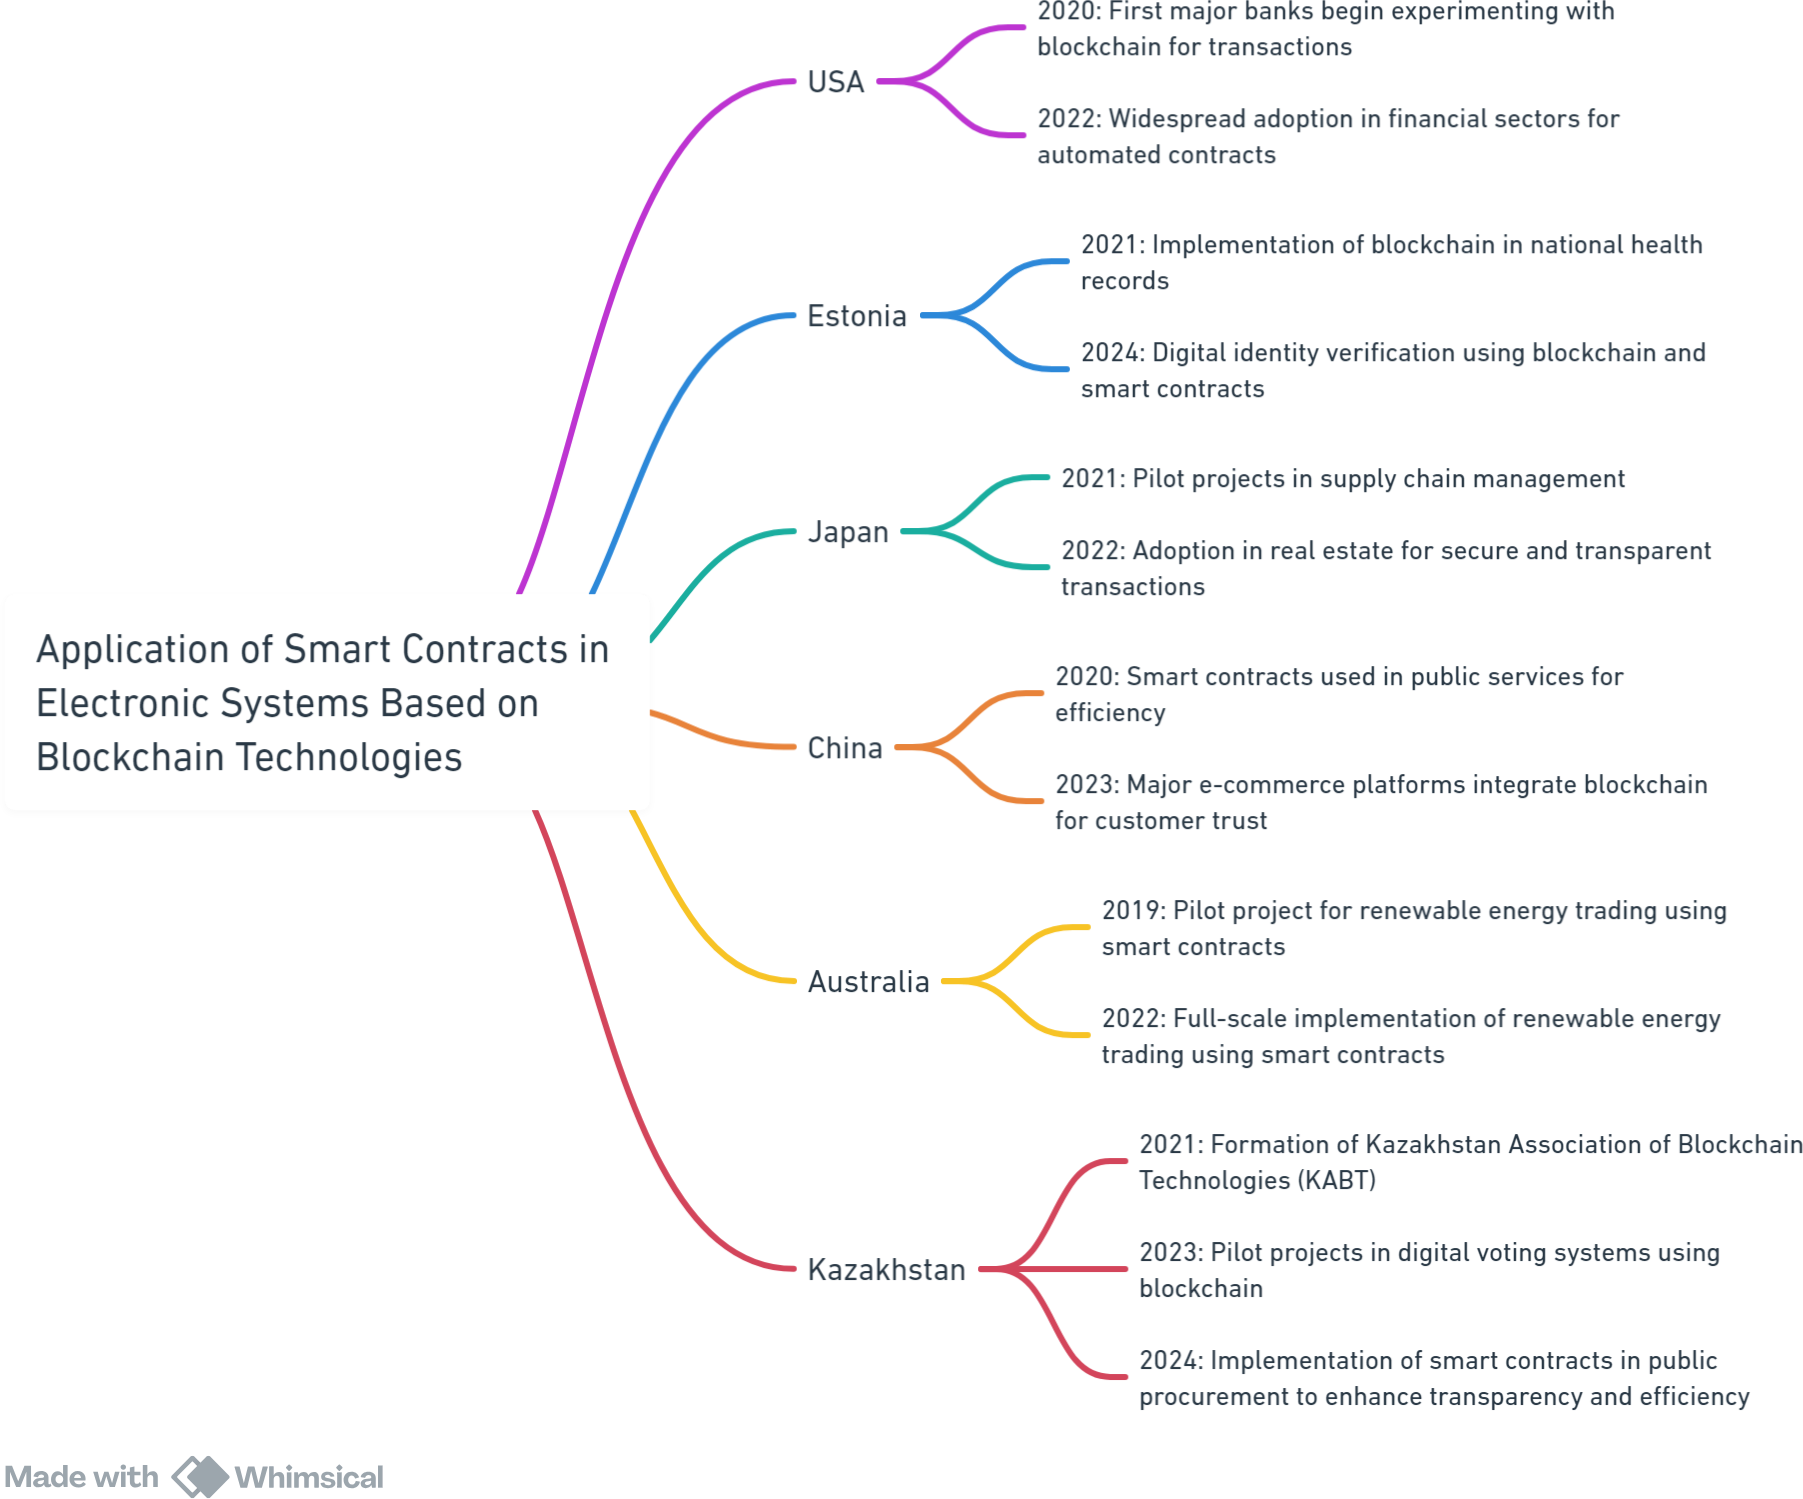
\includegraphics[width=0.8\textwidth]{assets/82}
	\caption*{}
\end{figure}

{\bfseries Fig.5- Global Adoption of Smart Contracts}

Figure 5 illustrates the utilization of smart contracts and it has
expanded beyond financial transactions to include sectors such as
digital identity verification, supply chain management, real estate,
public services, e-commerce, and renewable energy trading. This diverse
application range underscores the flexibility, security, and efficiency
benefits that smart contracts, powered by blockchain technology, offer.
The evolution and adoption of smart contracts over the years across
different countries signify a substantial shift towards more
transparent, efficient, and secure electronic systems in various
industries {[}15{]}. This technology not only promises to streamline
operations and reduce costs but also enhances trust and reliability in
digital transactions, marking a significant step forward in the digital
transformation of global industries.

Kazakhstan has emerged as a significant player in the global blockchain
landscape, especially in cryptocurrency mining and the adoption of
blockchain technologies. Following China\textquotesingle s crackdown on
cryptocurrency mining, Kazakhstan quickly became one of the top three
countries in the world for bitcoin mining, accounting for approximately
18\% of the global bitcoin hashrate by 2021. This rapid growth was
fueled by the country\textquotesingle s low electricity prices, which
attracted many mining operations. However, the influx of mining
activities also brought challenges, such as power outages and the need
for regulatory measures to manage energy consumption {[}16{]}.

In response to these challenges, Kazakhstan developed a comprehensive
legal framework to regulate digital assets and mining activities. The
"Law on Digital Assets," enacted in February 2023, provides clear
guidelines for licensing, taxation, and operation of digital mining and
digital asset exchanges. This legislation aims to ensure transparency
and compliance, mitigating the risks associated with unregulated mining
activities. It also introduces measures to curb illegal mining and
mandates transparent reporting and taxation of digital mining
activities. This proactive regulatory approach positions Kazakhstan as a
forward-thinking player in the global blockchain industry\hspace{0pt}
{[}17{]}.

Kazakhstan\textquotesingle s exploration of blockchain technology
extends beyond cryptocurrency mining. The country has initiated pilot
projects to implement blockchain-based voting systems, aiming to create
an immutable and verifiable ledger of votes. This initiative is part of
a broader effort to increase public trust in the electoral process and
reduce the risk of fraud. These projects align with the "Digital
Kazakhstan" state program, which seeks to leverage technology to improve
various sectors, including governance and public services.

To support the growing blockchain industry, Kazakhstan has launched
extensive educational programs in collaboration with Binance Academy.
These initiatives aim to train over 40,000 blockchain specialists by
2024, providing comprehensive education on blockchain engineering and
compliance. This focus on education underscores
Kazakhstan\textquotesingle s commitment to building a robust human
capital base to drive innovation and adoption of blockchain
technologies.

{\bfseries Conclusion.} The exploration of smart contracts within
blockchain technology reveals a significant potential to revolutionize
not only financial transactions but also critical societal functions
such as the electoral process. This article highlights how smart
contracts can automate and secure transactions with unparalleled
efficiency, transparency, and trust. Specifically, in the context of
electoral systems, smart contracts offer a transformative approach to
ensure secure, tamper-proof voting mechanisms, enhancing the integrity
and reliability of democratic elections. However, the journey towards
integrating smart contracts into electoral processes faces challenges,
including scalability, regulatory compliance, and technical
complexities. Despite these hurdles, the potential for smart contracts
to streamline electoral systems and reinforce democratic values through
improved security and transparency is immense. As blockchain technology
continues to evolve, its application in electoral processes promises to
usher in a new era of digital democracy, marked by enhanced electoral
integrity and public trust.

{\bfseries References}

1. Saim, M., Mamoon, M., Shah, I., \& Samad, A. (2022, November).
E-Voting via Upgradable Smart Contracts on Blockchain. In 2022
International Conference on Futuristic Technologies (INCOFT) (pp. 1-6).
IEEE. https://doi.org/10.1109/INCOFT55651.2022.10094482

2. Alvi, S. T., Uddin, M. N., \& Islam, L. (2020, August). Digital
voting: A blockchain-based e-voting system using biohash and smart
contract. //In 2020 third international conference on smart systems and
inventive technology (ICSSIT) (pp. 228-233). IEEE.
https://doi.org/10.1109/ICSSIT48917.2020.9214250

3. Baudier, P., Kondrateva, G., Ammi, C., \& Seulliet, E. Peace
engineering: The contribution of blockchain systems to the e-voting
process.//Technological Forecasting and Social Change.-2021.- Vol.162,
120397, https://doi.org/10.1016/j.techfore.2020.120396

4. Kaudare, A., Hazra, M., Shelar, A., \& Sabnis, M. (2020, June).
Implementing electronic voting system with blockchain technology.
//In~2020 International Conference for Emerging Technology IEEE. -
2020\emph{.-}p. 1-9. https://doi.org/10.1109/incet49848.2020.9154116

5. Al Barghuthi, N. B., Hamdan, I., Al Suwaidi, S., Lootah, A., Al
Amoudi, B., Al Shamsi, O., \& Al Aryani, S. (2019, November). An
analytical view on political voting system using blockchain
technology-uae case study. In~2019 Sixth HCT Information Technology
Trends (ITT\emph{)}~ IEEE.- 2019.- p. 132-137.
https://doi.org/10.1109/itt48889.2019.9075074

6. Kadam, P., Nikam, P., Raut, H., Hutke, S., \& Mathi, S. (2023, June).
Blockchain Based e-Voting System. //In~2023 3rd International Conference
on Intelligent Technologies (CONIT).-2023.- P.1-6. IEEE.
https://doi.org/10.1109/conit59222.2023.10205939

7. Jumagaliyeva A, Abdykerimova E, Turkmenbayev A, Muratova G., Talgat
A. Analysis of research on the implementation of Blockchain technologies
in regional electoral processes // International Journal of Electrical
and Computer Engineering (IJECE).- 2024.-Vol.14(3) - P.2854-2867
DOI:~http://doi.org/10.11591/ijece.v14i3.pp2854-2867

8. Gupta, S., Gupta, A., Pandya, I. Y., Bhatt, A., \& Mehta, K. (2023).
End to end secure e-voting using blockchain \& quantum key
distribution.//~MaterialsToday: Proceedings.-2023.- Vol.80(3).-P.
3363-3370. https://doi.org/10.1016/j.matpr.2021.07.254

9. Tripathi, G., Ahad, M. A., \& Casalino, G. (2023). A comprehensive
review of blockchain technology: Underlying principles and historical
background with future challenges. //Decision Analytics Journal.-
Vol.9.-2023, 100344. https://doi.org/10.1016/j.dajour.2023.100344

10. Almadani, M. S., Alotaibi, S., Alsobhi, H., Hussain, O. K., \&
Hussain, F. K. Blockchain-based multi-factor authentication: A
systematic literature review.~//Internet of Things,
100844.-Vol.23.-2023, 100844. https://doi.org/10.1016/j.iot.2023.100844

11. Khan, K. M., Arshad, J., \& Khan, M. M. (2021). Empirical analysis
of transaction malleability within blockchain-based
e-Voting.~//Computers \& Security.- 2021-Vol.100, 102081.
https://doi.org/10.1016/j.cose.2020.102081

12. Alam, S., Shuaib, M., Khan, W. Z., Garg, S., Kaddoum, G., Hossain,
M. S., \& Zikria, Y. B. (2021). Blockchain-based initiatives: current
state and challenges.~//Computer Networks.-2021, 108395.- Vol.198.
https://doi.org/10.1016/j.comnet.2021.108395

13. Kozhayeva, S., Rakhimzhanova, M., Ibrayeva, K., Muratova, G., \&
Dzhumagalieva, A. Formation of humanitarian qualities among students in
higher education institutions. //Astra Salvensis.- 2019.- Issue 13,
p.309-326. https://astrasalvensis.eu/2019-2

14. Alvi, S. T., Uddin, M. N., Islam, L., \& Ahamed, S. DVTChain: A
blockchain-based decentralized mechanism to ensure the security of
digital voting system voting system.~//Journal of King Saud
University-Computer and Information Sciences-2022.-~Vol.34(9).-P.
6855-6871. https://doi.org/10.1016/j.jksuci.2022.06.014

15. Nigmatov, A., Pradeep, A., \& Musulmonova, N. Blockchain Technology
in Improving Transparency and Efficiency in Government Operations.
//In~2023 15th International Conference on Electronics, Computers and
Artificial Intelligence (ECAI\emph{)}-2023.-P.01-06.
https://doi.org/10.1109/ecai58194.2023.10194154

16. Казахстанская ассоциация блокчейн-технологий и дата-центров (КАБТ),
"О нас", 2024. {[}Online{]}. Available: https://www.kabt.kz.
{[}Accessed: Jun. 20, 2024{]}.

17. A. B. Zeynelgabdin and E. E. Akhmetbek, "Блокчейн В Государственном
Управлении Казахстана," Public administration issues, vol. 3, pp.
111-134, 2021. {[}Online{]}. Available: http://vgmu.hse.ru. {[}Accessed:
Jun. 20, 2024{]}.

\emph{{\bfseries Information about the authors}}

Jumagaliyeva A.M.- senior lecturer, master of technical sciences,
K.Kulazhanov Kazakh University of Technology and Business, Astana,
Kazakhstan, e-mail: jumagalievaainur.m.@gmail.com;

Tulegulov A.D{\bfseries .-} сandidate of Physical and Mathematical
Sciences, Ass, Professor, K.Kulazhanov Kazakh University of Technology
and Business, Astana, Kazakhstan, e-mail: tad62@yandex.kz;

Murzabekova G.E.- сandidate of Physical and Mathematical Sciences, Ass.
Professor, S. Seifullin Kazakh Agrotechnical Research University,
Astana, Kazakhstan, e-mail: guldenmur07@mail.ru;

Muratova G.K.- сandidate of Physical and Mathematical Sciences, Ass.
Professor, S. Seifullin Kazakh Agrotechnical Research University,
Astana, Kazakhstan, e-mail: muratova@kazatu.edu.kz;

\emph{{\bfseries Информация об авторах}}

Джумагалиева А.М. - старший преподаватель, магистр технических наук,
Казахский университет технологий и бизнеса имени К.Кулажанова, Астана,
Казахстан, e-mail: jumagalievaainur.m.@gmail.com;

Тулегулов А.Д.- к.ф.-м.н., асс. профессор, Казахский университет
технологий и бизнеса им. К. Кулажанова, Астана, Казахстан, e-mail:
tad62@yandex.kz;

Мурзабекова Г.Е. - к.ф.-м.н, асс. профессор, Казахский агротехнический
исследовательский университет имени С.Сейфуллина, Астана, Казахстан,
e-mail: guldenmur07@mail.ru;

Муратова Г.К. - к.ф.-м.н., асс, профессор, Казахский агротехнический
исследовательский университет имени С.Сейфуллина, Астана, Казахстан,
e-mail: mugk@mail.ru
